\fancychapter[Efficient Marginalization of Discrete and Structured Latent Variables via Sparsity]{Efficient Marginalization of Discrete and Structured Latent Variables}
\label{chap:sparsemarg}

\cleardoublepage
\doublespacing

\noindent In this chapter, we focus on the objective of making neural models
more \textbf{compact}. We will propose a novel approach to train
discrete and structured latent variable models that achieves an exact
gradient unlike previous strategies in this field. Latent discrete
and structured variables are of particular interest for the compactness
of neural models since they can constrain the model and provide
inductive bias. This family of latent variable models can also be easily
semi-supervised, which can further increase the inductive bias and
thus the compactness of the model.

The exactness of the gradient of our approach is achieved through explicitly doing the
marginalization of \eqnref{eq:fit}. As we shall see, this computation turns out to be efficient thanks
to parameterizing the distribution over categories or structures with
\textbf{sparsity}. Therefore, while in the previous chapter we have
used sparsity for increased transparency, we will now use sparsity
for increased efficiency. Albeit in a different way than in the
previous chapter, this sparsity will too be \textbf{learned} over
time, increasing as the training progresses due to the model being
more confident on latent variable assignments.

\textit{This chapter is based on \citet*{correia2020procneurips}.}

\section{Motivation}
\label{sec:intro}

\noindent As discussed in \secref{sec:discrete_lvm_bg}, training with discrete latent variables can
become challenging, due to the need to compute a gradient of a large
sum over all possible latent variable assignments,
with each term
itself being potentially expensive (\eqnref{eq:fit}). This challenge is typically
tackled by estimating the gradient with Monte Carlo
methods~\citep[MC;][]{mohamed2019monte}, which rely on sampling
estimates. The two most common strategies for MC gradient estimation
are the score function
estimator~\citep[SFE;][]{rubinstein1976monte,paisley2012variational},
which suffers from high variance, or surrogate methods that rely on
the continuous relaxations, like straight-through~\citep{STE} or
Gumbel-Softmax~\citep{Concrete,GumbelSoftmax}, which potentially
reduce variance but introduce bias and modeling assumptions.

In this work, we take a step back and ask: Can we avoid sampling
entirely, and instead, deterministically evaluate the sum in \eqnref{eq:fit} with less
computation? To answer affirmatively, we propose an alternative
method to train these models by parameterizing the discrete
distribution with {\bf sparse
        mappings}\,---\,sparsemax~\citep{sparsemax} and two
structured counterparts, \smap~\citep{sparsemap} and a
novel mapping top-$k$ sparsemax. Sparsity implies that some
assignments of the latent variable are entirely ruled out. This leads
to the corresponding terms in the sum evaluating trivially to zero,
allowing us to disregard potentially expensive computations.

\paragraph*{Contributions.} We introduce a general strategy for
learning discrete latent variable models that hinges on
learning a sparse distribution over the possible assignments. In the
unstructured categorical case, our strategy relies on the sparsemax
activation function, presented in~\secref{sec:categorical}, while in the
structured case we propose two strategies, \smap and top-$k$
sparsemax, presented in~\secref{sec:structured}. Unlike existing
approaches, our strategies involve neither MC estimation nor any
relaxation of the discrete latent variable to the continuous space.
We demonstrate our strategy in three different applications: a
semi-supervised generative model, an emergent communication game, and
a bit-vector variational auto-encoder. We provide a thorough analysis
and comparison to MC methods, and\,---\,when feasible\,---\,to exact
marginalization. Our approach is consistently a top performer,
combining the accuracy and robustness of exact marginalization with
the efficiency of single-sample estimators.

\section{Previous Work}

\paragraph*{Differentiable sparse mappings.} There has been recent
interest in applying sparse mappings (see \secref{sec:sparsity_background}) of discrete distributions in
deep discriminative models~\citep{sparsemax,
    sparsemap, fusedmax, entmax, sparsemapcg}, attention
mechanisms~\citep{malaviya2018sparse, shao2019ssn,
    maruf2019selective, correia2019adaptively}, and in topic
models~\citep{caothesis}. Our work focuses on the parameterization of
distributions over latent variables with sparse mappings, on the
computational advantage to be gained by sparsity, and on the contrast
between our novel training method and common sampling-based methods.

\paragraph*{Reducing sampling noise.} The sampling procedure found in
SFE is a great source of variance in models that use it.
To reduce this variance, many works have proposed
baselines~\citep{Williams1992,MuProp,CV2013}. VIMCO~\citep{VIMCO} is
a multi-sample estimator which exploits variance reduction via
input-dependent baselines as well as a lower bound on marginal
likelihood which is tighter than the ELBO~\citep{IWAE}. The number of
samples in VIMCO is a hyperparameter that stays fixed throughout
training. Our methods, in contrast, may take several decoder calls
initially, but that number automatically decreases over time as
training progresses. While baselines must be independent of the
sample for which we assess the score function, exploiting correlation
in the downstream losses of dependent samples holds potential for
further variance reduction. These are known as control
variates~\citep{GreensmithEtAl}. REBAR~\citep{REBAR} exploits a
continuous relaxation to obtain a dependent sample and uses the
downstream loss assessed at the relaxed sample to define a control
variate. RELAX~\citep{RELAX}, instead, learns to predict the
downstream loss of the relaxed sample with an auxiliary network. In
contrast, sparse marginalization works for any factorization where a
primitive for $1$-best (or $k$-best) enumeration is available and
takes no additional parameters nor additional optimization
objectives. Another line of work approximates $\argmax$ gradients by
perturbed finite differences \cite{lorberbom2019direct,vlastelica};
this requires the same computation primitive as our approach but is
always biased. ARM~\citep{yin2019arm} is a control variate based on
antithetic samples~\citep{mcbook}: it does not require relaxation nor
additional parameters, but it only applies to factorial Bernoulli
distributions. Closest to our work are variance reduction techniques
that rely on partial marginalization, typically of the top-$k$
assignments to the latent variable~\citep{RB19,Kool2020Estimating}.
These methods show improved performance and variance reduction, but
require rejection sampling, which can be challenging in structured
problems.

\section{Efficient Marginalization via Sparsity}
\label{sec:categorical}

\noindent As discussed in \secref{sec:lvm}, the challenge of computing the
exact expectation in \eqnref{eq:fit} is linked to the need to compute
a sum with a large number of terms. This holds when the probability
distribution over latent assignments is {\it dense} ({\it i.e.},
every assignment $z \in \ZZ$ has non-zero probability), which is
indeed the case for most parameterizations of discrete distributions.
Our proposed methods hinge on {\it sparsifying} this sum.

Take the example where $\mathcal Z = \{1, \ldots, K\}$, with a neural
network predicting from $x$ to a $K$-dimensional vector of real-valued
scores $\s = \g(x; \theta)$, such that $s_z$ is the score of
$z$.\footnote{Not to be confused with ``score function,'' as in SFE,
    which refers to the gradient of the log-likelihood.} The traditional
way to obtain the vector $\pv$ parameterizing $\pi(z|x;\theta)$ is
with the softmax transform (\ie, $\pv = \softmax(\s)$). Since this
gives $\pi(z|x;\theta) \propto \exp(s_z)$, the expectation in
\eqnref{eq:fit} depends on $\ell(x, z; \theta)$ for every possible
$z$.

We rethink this standard parameterization, proposing a
\textbf{sparse} mapping from scores to the simplex. In particular, we
substitute the softmax activation function by
sparsemax~\citep{sparsemax}, described in
\secref{sec:sparsity_background}.

Our main insight is that with a sparse parameterization of $\pi$, we
can compute the expectation in \eqnref{eq:fit} evaluating $\ell(x, z;
    \theta)$ only for assignments $z \in \bar\ZZ \defeq \{z : \pi(z | x,
    \theta) > 0\}$. This leads to a powerful alternative to MC
estimation, which requires fewer than $|\ZZ|$ evaluations of $\ell$,
and which strategically\,---\,yet deterministically\,---\,selects
which assignments $\bar\ZZ$ to evaluate $\ell$ on. Empirically, our
analysis in \secref{sec:applications} reveals an adaptive behavior of
this sparsity-inducing mechanism, performing more loss evaluations in
early iterations while the model is uncertain, and quickly reducing
the number of evaluations, especially for unambiguous data points.
This is a notable property of our learning strategy: In contrast, MC
estimation cannot decide when an ambiguous data point may require
more sampling for accurate estimation; and directly evaluating
\eqnref{eq:fit} with the dense $\pv$ resulting from a softmax
parameterization never reduces the number of evaluations required,
even for simple instances.

\section{\label{sec:structured}Structured Latent Variables}

\noindent As discussed in \secref{sec:struct_lvm_bg}, many interesting models
can include latent variables that exist in a set of combinatorial
size. While it may be tempting to consider using sparsemax to avoid
the expensive sum in the exact expectation of \eqnref{eq:fit}, this
is prohibitive too: solving the problem in \eqnref{eq:sparsemax}
still requires explicit manipulation of the large vector $\bm{s} \in
    \mathbb{R}^{|\ZZ|}$, and even if we could avoid this, in the worst
case ($\bm{s}=\bm{0}$) the resulting sparsemax distribution would
still have exponentially large support. Fortunately, we show next
that it is still possible to develop sparsification strategies to
handle the combinatorial explosion of $\ZZ$ in the structured case.
We propose two different methods to obtain a sparse distribution
$\pv$ supported only over a bounded-size subset of $\ZZ$: top-$k$
sparsemax (\secref{sec:topksparse}) and \smap (\secref{sec:smap}).

\subsection{\label{sec:topksparse}\texorpdfstring{Top-{\boldmath $k$}}{Top-k} Sparsemax}

\noindent Recall that the sparsemax operator (\eqnref{eq:sparsemax}) is simply
the Euclidean projection onto the $|\ZZ|$-dimensional probability
simplex. While there is a propensity for sparsity, there is no upper
bound on the number of non-zeros of the resulting distribution. When
$\ZZ$ is large, one possibility is to add a cardinality constraint
$\|\pv\|_0 \le k$ for some prescribed $k \in \mathbb{N}$. The
resulting problem becomes
%
\begin{equation}\label{eq:topk_sparsemax}
    \sparsemaxk(\s) \coloneqq
    \argmin_{\pv \in \simplex^{|\ZZ|-1}, \, \|\pv\|_0 \le k} \| \pv - \s \|_2^2,
\end{equation}
%
which is known as a \emph{sparse projection onto the simplex} and has
been studied in detail by \citet{kyrillidis2013sparse} and used to
smooth structured prediction
losses~\citep{NIPS2018_7726,blondel2020}. Remarkably, while this is a
non-convex problem, its solution $\pv^\star$ can be written as a
composition of two functions: a top-$k$ operator $\topk:
    \mathbb{R}^{|\ZZ|} \rightarrow \mathbb{R}^{|\ZZ|}$, which returns a
vector identical to its input but where all the entries not among the
$k$ largest ones are masked out (set to $-\infty$), and the
$k$-dimensional sparsemax operator.

Formally, $\sparsemaxk = \sparsemax(\topk(\s))$. Being a composition
of operators, its Jacobian becomes a product of matrices and hence
simple to compute.\footnote{the Jacobian of $\topk$ is a diagonal matrix whose
    diagonal is a multi-hot vector indicating the top-$k$ elements of
    $\s$}

To apply the top-$k$ sparsemax to a large or combinatorial set $\ZZ$,
all we need is a primitive to compute the top-$k$ entries of
$s$\,---\,this is available for many structured problems (for example,
sequential models via $k$-best dynamic programming) and, when $\ZZ$
is the set of joint assignments of $D$ discrete binary variables, it
can be done with a cost $\mathcal{O}(kD)$.

After enumerating this set, we parameterize $\pi(z|x;\theta)$ by
applying sparsemax to that top-$k$, with a
computational cost $\mathcal{O}(k)$. Note that {\bf this method is
        identical to sparsemax whenever $\|\sparsemax(\s)\|_0 \le k$}: if
during training the model learns to assign a sparse distribution to
the latent variable, we are effectively using a sparsemax
parameterization as presented in \secref{sec:categorical} with cheap
computation. In fact, the solution of \eqnref{eq:topk_sparsemax}
gives us a certificate of optimality whenever $\|\pv^\star\|_0 < k$.

\subsection{\label{sec:smap}\smap}

\noindent A second possibility to obtain efficient summation over a
combinatorial space without imposing any constraints on $\ell(x, z;
    \theta)$ is to use \smap~\citep[\secref{sec:smap_bg};][]{sparsemap, sparsemapcg}.
Due to the properties of \smap,
assessing the expectation in \eqnref{eq:fit} only requires evaluating
$|\bar\ZZ| = \mathcal{O}(D)$ terms.

\section{\label{sec:applications}Experimental Analysis}

\noindent We next demonstrate the applicability of our proposed strategies by
tackling three tasks: a deep generative model with semi-supervision
(\secref{sec:gen}), an emergent communication two-player game over a
discrete channel (\secref{sec:comm}), and a variational auto-encoder with
latent binary factors (\secref{sec:bernvae}).

We follow the experimental procedures described in~\citep{RB19}
and~\citep{Lazaridou2017} for~\secref{sec:gen} and \secref{sec:comm},
respectively. We describe the most relevant training details and key
differences in architectures when applicable. For other
implementation details that we do not mention here, we refer the
reader to the works referenced above. For all Gumbel baselines, we
relax the sample into the continuous space but assume a discrete
distribution when computing the entropy of $\pi(z |x; \theta)$, as
suggested as one implementation option in \citet{Concrete}. Our code
is publicly available\footnote{
    \url{https://github.com/deep-spin/sparse-marginalization-lvm}} and
was largely inspired by the structure and implementations found in
EGG~\citep{Kharitonov2019}, having been built upon it.

\subsection{Semi-Supervised Variational Auto-Encoder}\label{sec:gen}

\noindent We consider the semi-supervised Variational Auto-Encoder
(VAE) of \citet{KingmaEtAl2014SSVAE}, which models the joint
probability
%
\begin{equation}
    p_{XZH}(z,h,x|\phi)=p_Z(z)p_H(h)p_{X|ZH}(x|z,h)\,,
\end{equation}
%
where $x$ is an
observation (an MNIST image), $h$ is a continuous latent variable
with a $n$-dimensional standard Gaussian prior, and $z$ is a discrete
random variable with a uniform prior over $K$ categories.

The semi-supervised objective is
%
\begin{equation}
    L_{\mathcal D}(\phi) = - \log p_X(x | \phi) - \log p_{XZ}(x, z | \phi) + \mathcal{R}(\phi),
    \label{eq:ss_loss_vae}
\end{equation}
%
where $\mathcal{R}(\phi)$ is a regularizer we will specify below, and
$\log p_X(x | \phi)$ and $\log p_{XZ}(x, z | \phi)$ is the log-likelihood
of the unsupervised and supervised components, respectively.

For the unsupervised component of the loss, note that the marginal likelihood
%
\begin{equation}
    p_X(x | \phi) = \sum_{z=1}^K \int_h p_{X|ZH}(x | z, h; \phi)p_H(h)p_Z(z) \dd h
\end{equation}
%
is intractable, due to the marginalization of $h \in \mathbb R^n$.
For the same reason, the marginal likelihood of the supervised
component of the loss $p_{XZ}(x, z | \phi)$ is also intractable.
Additionally, on the unsupervised component, for a fixed $h$ (\eg,
sampled), marginalizing $z$ requires $K$ calls to the decoder, which
can be costly depending on its architecture.

To circumvent the need for the marginal likelihood,
\citet{KingmaEtAl2014SSVAE} use variational inference
\citep{Jordan+1999:VI} with an approximate posterior $\pi(z|x;
    \theta_\pi)q(h|z,x; \lambda)$. This trains a classifier $\pi(z|x;
    \theta_\pi)$ along with the generative model. In
\citet{KingmaEtAl2014SSVAE}, $h$ is sampled with the
reparameterization trick~\citep{Kingma+2014:VAE,RezendeEtAl14VAE},
and the expectation over $z$ is computed in closed-form, that is,
assessing all $K$ terms of the sum for a sampled $h$. Under the
notation in \secref{sec:lvm}, and for the unsupervised component of
the loss in \eqnref{eq:ss_loss_vae}, we let $\theta_\ell = \{\lambda,
    \phi\}$ and define $\pi(z|x; \theta_\pi) \defeq q(z|x; \lambda)$ and
%
\begin{align}
    \begin{split}
        \ell(x, z; \theta_\ell) \defeq
        & - \mathbb E_{q(h|z,  \lambda)}\left[ \log p_{X|ZH}(x |z, h; \phi) \right] \\
        & - \log \frac{p_Z(z)}{\pi(z |x; \theta_\pi)}                          \\
        & + \KL\left[q(h |x, z; \lambda) \,\,\|\,\, p_H(h)\right],
        \label{eq:elbonotation}
    \end{split}
\end{align}
%
which turns \eqnref{eq:fit} into the (negative) evidence lower bound
(ELBO). For the supervised component in \eqnref{eq:ss_loss_vae} we let
%
\begin{align}
    \begin{split}
        \ell(x, z; \theta_\ell) \defeq
        & - \mathbb E_{q(h|z,  \lambda)}\left[ \log p_{X|ZH}(x |z, h; \phi) \right] \\
        & - \log p_Z(z)                          \\
        & + \KL\left[q(h |x, z; \lambda) \,\,\|\,\, p_H(h)\right].
        \label{eq:elbosupervised}
    \end{split}
\end{align}
%
Finally, to complete the specification of \eqnref{eq:ss_loss_vae},
we let $\mathcal R(\phi) = - \log \pi(z |x; \theta_\pi)$ when $z$ is supervised
in order to train the classifier on the supervised data as well.
To update $q(h | x, z; \lambda)$, we use the
reparameterization trick to obtain gradients through a sampled $h$.
For $\pi(z | x; \theta_\pi)$, we may still explicitly marginalize over
each possible assignment of $z$, but this has a multiplicative cost
on $K$. As an alternative, we parameterize $\pi(z|x,
    \theta_\pi)$ with a sparse mapping, comparing it to the original
formulation and with stochastic gradients based on SFE and continuous
relaxations of $z$.

\begin{figure}[htbp]
    \centering
    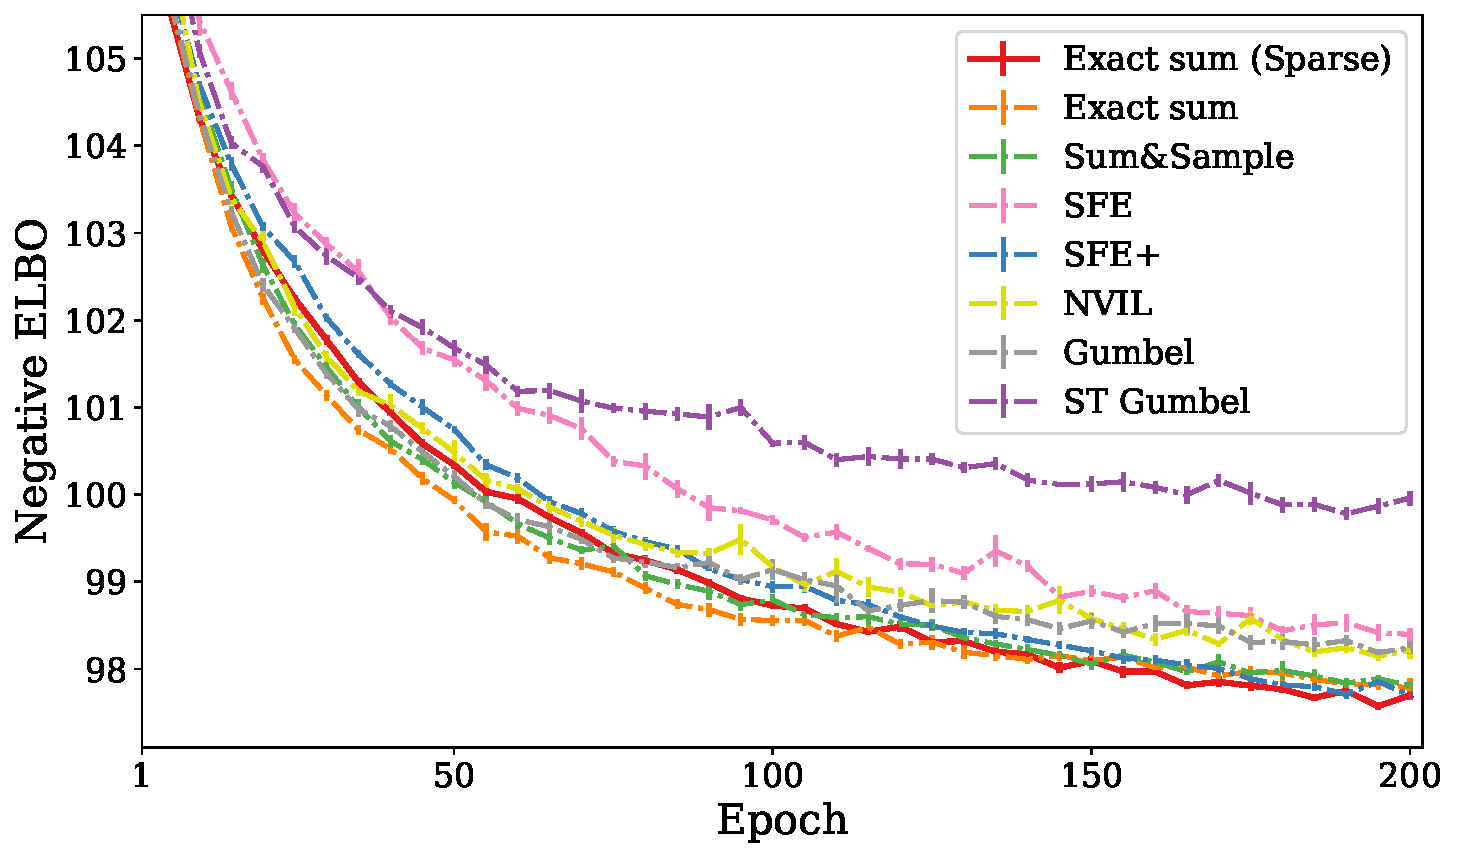
\includegraphics[width=.9\textwidth]{Figures/ss_mnist_elbo_path.pdf}
    \caption{\label{fig:ssvaeelbo}Learning curves on the test set for semi-supervised VAE on MNIST.}
\end{figure}

\begin{table}[t]
    \centering
    \tlfstyle
    \begin{tabular}{lrr}
        \toprule
        Method &
        Accuracy (\%)
               & Decoder calls                                                \\
        \midrule

        \multicolumn{3}{l}{\emph{Monte Carlo}}                                \\
        SFE
               & 94.75{\color{gray}$\pm$ .002} & 1                            \\
        SFE$+$
               & 96.53{\color{gray}$\pm$ .001} & 2                            \\
        NVIL
               & 96.01{\color{gray}$\pm$ .002} & 1                            \\
        Sum\&Sample
               & 96.73{\color{gray}$\pm$ .001} & 2                            \\
        Gumbel
               & 95.46{\color{gray}$\pm$ .001} & 1                            \\
        ST Gumbel
               & 86.35{\color{gray}$\pm$ .006} & 1                            \\
        \spacerule
        \multicolumn{3}{l}{\emph{Marginalization}}                            \\
        Dense
               & 96.93{\color{gray}$\pm$ .001} & 10                           \\
        Sparse {\small \color{gray}{(proposed)}}
               & 96.87{\color{gray}$\pm$ .001} & 1.01{\color{gray}$\pm$ 0.01} \\
        \bottomrule
    \end{tabular}
    \caption[Test set results for semi-supervised VAE on MNIST.]{\label{tab:ssvaeelbo}
        Average test results and standard errors over 10 runs for semi-supervised VAE on MNIST.}
\end{table}

\paragraph*{Data and architecture.} We evaluate this model on the
MNIST dataset~\citep{lecun1998gradient}, using 10\% of labeled data,
treating the remaining data as unlabeled. MNIST consists of $28
    \times 28$ gray-scale images of hand-written digits. It contains
60K data points for training and 10K for testing. We
perform model selection on the last 10K data points of the training
split. In this experiment, the classification network consists of
three fully connected hidden layers of size 256, using ReLU
activations. The generative and inference network both consist of one
hidden layer of size 128, also with ReLU activations. The
multivariate Gaussian has 8 dimensions and its covariance is
diagonal. For all models we have chosen the learning rate based on
the best ELBO on the validation set, doing a grid search (5e-5, 1e-4,
5e-4, 1e-3, 5e-3). The accuracy shown in \tableref{tab:ssvaeelbo} is
the test accuracy taken after the last epoch of training. The
temperature of the Gumbel models was annealed according to $\tau =
    \max\left(0.5, -rt\right)$, where $t$ is the global training step.
For these models, we also did a grid search over $r$ (1e-5, 1e-4) and
over the frequency of updating $\tau$ every (500, 1000) steps.
Optimization was done with Adam. For our method, in the labeled loss
component of the semi-supervised objective, we used the sparsemax
loss~\citep{sparsemax}. Following \citet{RB19}, we pre-train
the network with only labeled data before training with the whole
training set. Likewise, for our method, we pre-trained the network on
the sparsemax loss and every other method with the Negative
Log-Likelihood loss. Each model was trained for 200 epochs.

\paragraph*{Comparisons.} Our proposal's key ingredient is sparsity,
which permits exact marginalization and a deterministic gradient. To
investigate the impact of sparsity alone, we report a comparison
against the exact marginalization over the entire support of $\ZZ$ using
a dense softmax parameterization. To investigate the impact of
deterministic gradients, we compare to stochastic gradients:

\begin{itemize}
    \item SFE with a moving average baseline;
    \item SFE with a self-critic
          baseline~\citep[SFE+;][]{rennie2017self}, that is, we use $\log
              p_{X|ZH}(x|z', h; \phi)$ as baseline, where $z' \sim \pi(z|x; \theta_\pi)$
          is an independent sample;
    \item NVIL~\citep{mnih2014neural}
          with a learned baseline (we train an MLP to predict the learning
          signal by minimizing mean squared error);
          \footnote{NVIL and SFE+ are
              similar, the difference being that the baseline in SFE+ does not
              require additional parameters nor does it introduce additional
              objectives.}
    \item Sum-and-sample~\citep{RB19};
    \item Gumbel-Softmax, which relaxes the random variable to the interior of the simplex;
    \item ST Gumbel-Softmax, which discretizes the relaxation in
          the forward pass, but ignores the discretization function in the
          backward pass.\footnote{For Gumbel-Softmax (with and
              without ST), we follow \citet{GumbelSoftmax} and substitute
              $\KL(\pi(z|x; \theta_\pi) \| p_Z(z))$ in the ELBO by the $\KL$
              divergence of $\Cat(\softmax(\s))$ from a discrete uniform prior.
              Strictly speaking, this means the objective is not a proper ELBO and
              its relationship to an ELBO is unclear~\citep[Appendix
                  C.2]{Concrete}.}
\end{itemize}

\paragraph*{Results and discussion.}
In \figref{fig:ssvaeelbo}, we see that our proposed sparse
marginalization approach performs just as well as its dense
counterpart, both in terms of ELBO and accuracy. However, by
inspecting the number of times each method calls the decoder for
assessments of $p_{X|ZH}(x|z, h;\phi)$, we can see that the effective
support of our method is much smaller\,---\,sparsemax-parameterized
posteriors get very confident, and mostly require one, and sometimes
two, calls to the decoder. Regarding the Monte Carlo methods, the
continuous relaxation done by Gumbel-Softmax underperformed all the
other methods, except for SFE with a moving average. While
SFE+ and Sum\&Sample are very strong performers, they will always
require throughout training the same number of calls to the decoder
(in this case, two). On the other hand, sparsemax makes a small
number of decoder calls not due to a choice in hyperparameters but
thanks to the model converging to only using a small support, which
can endow this method with a lower number of computations as it
becomes more confident.

\subsection{Emergent Communication Game}\label{sec:comm}

\noindent Emergent communication studies how two agents can develop a
communication protocol to solve a task
collaboratively~\citep{kirby2002natural}. Recent work used neural
latent variable models to train these agents via a ``collaborative
game'' between
them~\citep{Lazaridou2017,Havrylov2017,
    jorge2016learning, foerster2016learning, sukhbaatar2016learning}. In
\citet{Lazaridou2017}, one of the agents, the \emph{sender}, sees an
image $v_y$ and sends a single symbol message $z$ chosen from the \emph{vocabulary} set
$\mathcal{Z}$ to the other agent, the
\emph{receiver}, who needs to choose $v_y$ out of
a set of images $\mathcal{V} = \left\{ v_1, \dots, v_C
    \right\}$.\footnote{\citet{Lazaridou2017} lets the sender see the
    full set $\mathcal{V}$. However, we follow \citet{Havrylov2017}
    in showing only the correct image $v_y$ to the sender, making the
    game harder, as the message $z$ needs to encode a good
    ``description'' of $v_y$ instead of encoding only
    its differences from $\mathcal{V}\setminus \{v_y\}$.} They found that
the messages communicated this way can be correlated with broad
object properties amenable to interpretation by humans. In our
framework of \eqnref{eq:fit}, we let $x = (\mathcal{V}, y)$ and define
$\ell (x, z; \theta) \coloneqq -\log p_{X|Z}(y |\mathcal{V}, z; \theta_\ell)$
and
$\pi (z |x; \theta) \coloneqq p_{Z|X}(z |v_y; \theta_\pi)\,$,
where
$p_{X|Z}(y |\mathcal{V}, z; \theta_\ell)$ corresponds to the sender and
$p_{Z|X}(z |v_y; \theta_\pi)$ to the receiver. Following
\citet{Lazaridou2017}, we add an entropy regularization of $\pi (z
    |x; \theta)$ to the loss, with a coefficient as an
hyperparameter~\citep{Mnih2016}.

\paragraph*{Data and architecture.} In this application, we closely
followed the experimental procedure described
by~\citet{Lazaridou2017} with a few key differences. The architecture
of the sender and the receiver is identical with the exception that
the sender does not take as input the distracting images along with
the correct image\,---\,only the correct image. To make the game even
harder, we increase the collection of images $|\mathcal{V}|$ as
suggested by \citet{Havrylov2017}; in our experiments, we increase it
from 2 to 16. and the vocabulary of the sender was increased to 256.
The hidden size and embedding size were also increased to 512 and 256,
respectively. We did a grid search on the learning rate (0.01, 0.005,
0.001) and entropy regularizer (0.1, 0.05, 0.01) and chose the best
configuration for each model on the validation set based on the
communication success. For the Gumbel models, we applied the same
schedule and grid search to the temperature as described in
\secref{sec:gen}. All models were trained with the Adam optimizer,
with a batch size of 64 and during 200 epochs. We choose the
vocabulary of the sender to be 256, the hidden size to be 512 and the
embedding size to be 256. All methods are trained for 500 epochs. The
data used by \citet{Lazaridou2017} is a subset of ImageNet containing
463,000 images, chosen by sampling 100 images from 463 base-level
concepts. The images are then applied a forward-pass through the
pre-trained VGG ConvNet~\citep{convnet} and the representations at the
second-to-last fully connected layer are saved to use as input to the
sender/receiver.

\paragraph*{Comparisons.} We compare our method to stochastic gradient
estimators as well as exact marginalization under a dense softmax
parameterization of $p_{Z|X}(z |v_y; \theta_\pi)$. Again, we have
unbiased (SFE with moving average baseline, SFE+, and NVIL) and
biased (Gumbel-Softmax and ST Gumbel-Softmax) estimators. For SFE we
also experiment using a 0/1 loss.

\begin{table}[t]
    \begin{center}
        \tlfstyle
        \begin{tabular}{lrrr}
            \toprule
            Method                                 & \multicolumn{2}{r}{Communication success (\%)}                                                        & Decoder calls                                                          \\
            \midrule
            {\emph{Monte Carlo}}                   &                                                                                                       &                                     &                                  \\
            SFE (NLL)                              & 33.05\!\!\!\!\!\!\!\!\!\!\!\!\!\!\!\!\!\!\!\!\!\!\!\!\!\!\!\!\!\!\!\!\!\!\!\!\!\!\!\!\!\!\!\!\!\!\!\! & {\color{gray}$\pm$ \phantom{1}2.84} & 1                                \\
            SFE (0/1)                              & 55.36\!\!\!\!\!\!\!\!\!\!\!\!\!\!\!\!\!\!\!\!\!\!\!\!\!\!\!\!\!\!\!\!\!\!\!\!\!\!\!\!\!\!\!\!\!\!\!\! & {\color{gray}$\pm$ \phantom{1}2.92} & 1                                \\
            SFE$+$ (0/1)                           & 44.32\!\!\!\!\!\!\!\!\!\!\!\!\!\!\!\!\!\!\!\!\!\!\!\!\!\!\!\!\!\!\!\!\!\!\!\!\!\!\!\!\!\!\!\!\!\!\!\! & {\color{gray}$\pm$ \phantom{1}2.72} & 2                                \\
            NVIL                                   & 37.04\!\!\!\!\!\!\!\!\!\!\!\!\!\!\!\!\!\!\!\!\!\!\!\!\!\!\!\!\!\!\!\!\!\!\!\!\!\!\!\!\!\!\!\!\!\!\!\! & {\color{gray}$\pm$ \phantom{1}1.61} & 1                                \\
            Gumbel                                 & 23.51\!\!\!\!\!\!\!\!\!\!\!\!\!\!\!\!\!\!\!\!\!\!\!\!\!\!\!\!\!\!\!\!\!\!\!\!\!\!\!\!\!\!\!\!\!\!\!\! & {\color{gray}$\pm$ 16.19}           & 1                                \\
            ST Gumbel                              & 27.42\!\!\!\!\!\!\!\!\!\!\!\!\!\!\!\!\!\!\!\!\!\!\!\!\!\!\!\!\!\!\!\!\!\!\!\!\!\!\!\!\!\!\!\!\!\!\!\! & {\color{gray}$\pm$ 13.36}           & 1                                \\
            \spacerule
            \emph{Marginalization}                 &                                                                                                       &                                     &                                  \\
            Dense                                  & 93.37\!\!\!\!\!\!\!\!\!\!\!\!\!\!\!\!\!\!\!\!\!\!\!\!\!\!\!\!\!\!\!\!\!\!\!\!\!\!\!\!\!\!\!\!\!\!\!\! & {\color{gray}$\pm$ \phantom{1}0.42} & 256                              \\
            Sparse {\small \color{gray}(proposed)} & 93.35\!\!\!\!\!\!\!\!\!\!\!\!\!\!\!\!\!\!\!\!\!\!\!\!\!\!\!\!\!\!\!\!\!\!\!\!\!\!\!\!\!\!\!\!\!\!\!\! & {\color{gray}$\pm$ \phantom{1}0.50} & 3.13\,\,{\color{gray}$\pm$ 0.48} \\
            \bottomrule
        \end{tabular}
    \end{center}
    \caption[Emergent communication success test results.]{Emergent communication success test results,
        averaged across 10 runs. Random guess baseline 6.25\%.}
    \label{tab:symbol}
\end{table}

\paragraph*{Results and discussion.}
Table~\ref{tab:symbol} shows the communication success (accuracy of
the receiver at picking the correct image $v_y$). While the
communication success for $|\mathcal{V}|=2$ in \citet{Lazaridou2017}
was close to perfect, we see that increasing $|\mathcal{V}|$ to 16
makes this game much harder to sampling-based approaches.
Only the models that do explicit marginalization achieve close to
perfect communication in the test set. However, as $\ZZ$ increases,
marginalizing with a softmax parameterization gets computationally
more expensive, as it requires $|\ZZ|$ forward and backward passes on
the receiver. Unlike softmax, the model trained with sparsemax
gives very small support, requiring on average only 3 decoder
calls. In fact, sparsemax
starts off dense while exploring, but quickly becomes very sparse
(\figref{fig:nonzero_comm}).

\begin{figure*}[ht]
    \centering
    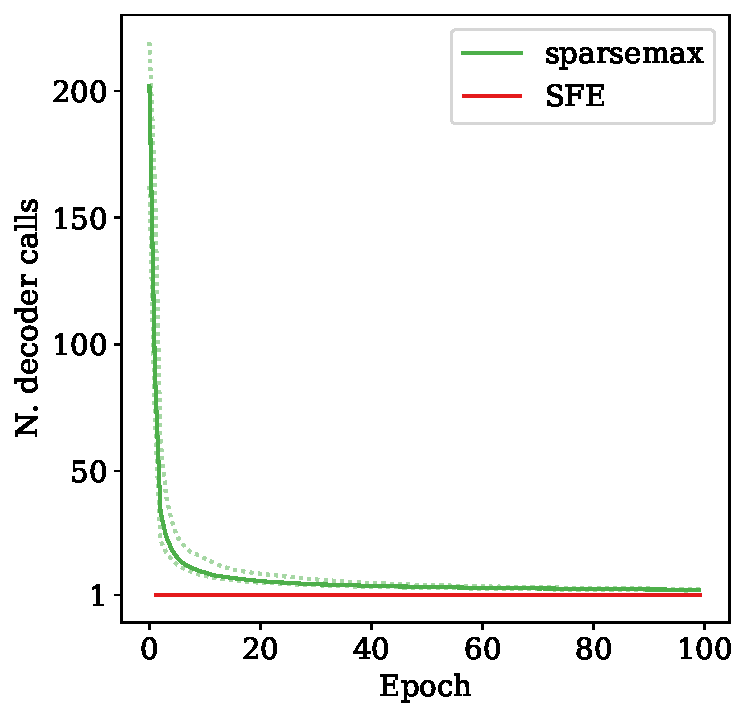
\includegraphics[width=0.65\columnwidth]{Figures/sparsemax_nonzero_em_comm.pdf}
    \caption[Median decoder calls per epoch.]{
        Median decoder calls per epoch during training
        time with 10 and 90 percentiles in dotted lines by sparsemax.
    }
    \label{fig:nonzero_comm}
\end{figure*}

\subsection{Bit-Vector Variational Auto-Encoder}\label{sec:bernvae}

\noindent As described in \secref{sec:structured},
combinatorial interactions and constraints will make $\ZZ$ exponentially
large. In this section, we study the illustrative case of encoding
images into a binary codeword $z$, by training a latent
bit-vector variational auto-encoder~\citep{GumbelSoftmax,
    mnih2014neural}. One approach for parameterizing the approximate
posterior is to use a Gibbs distribution, decomposable as a product
of independent Bernoulli,
%
\begin{equation}
    q(z |x; \lambda) \propto\exp(\DP{\bm{a}_z}{\bm{t}}) = \prod_{i=1}^D q(z_i |x; \lambda)\,,
\end{equation}
%
with each $z_i$ being a Bernoulli with parameter $t_i$, and $D$ being
the size of the bit-vector. While marginalizing over all the
possible $z$ is intractable, drawing samples can be done
efficiently by sampling each component independently, and the entropy
has a closed-form expression.
This efficient sampling and entropy computation relies on an independence
assumption; in general, we may not have access to such efficient
computation.

Training this VAE to minimize the negative ELBO corresponds to
%
\begin{equation}
    \ell(x, z; \theta_\ell) \defeq - \log \frac{p_{XZ}(x, z | \phi)}{q(z | x, \lambda)}\,;
\end{equation}
%
we use a uniform prior $p_Z(z)=1/|\ZZ|=1/{2^D}$. This
objective does not constrain $\pi(z| x;\theta_\pi) \defeq q(z |x,
    \lambda)$ to the Gibbs parameterization, and thus to apply our
methods we will differ from it.

\paragraph*{Top-{\boldmath $k$} sparsemax parameterization.} As pointed
out in \secref{sec:structured}, we now cannot explicitly handle the
sparsemax mapping $\pv = \sparsemax(\s)$, as it
involves a vector of dimension $2^D$. However, given $\bm{t}$, we can
efficiently find the $k$ largest configurations in time
$\mathcal{O}(kD)$, with the procedure described in
\secref{sec:topksparse}, and thus we can evaluate $\sparsemaxk(\s)$
efficiently.

\paragraph*{\smap parameterization.} Another sparse alternative to the
intractable structured sparsemax, as discussed in
\secref{sec:structured}, is \smap. In this case, we compute an optimal
distribution $\pv$ using the active set algorithm of
\citet{sparsemap}, by using a maximization oracle which
can be computed in $\mathcal{O}(D)$:
\begin{equation}
    \argmax_z \DP{\bm{a}_z}{\bm{t}} = z^\star \quad \text{s.t.}\quad
    [\bm{a}_{z^\star}]_i = \begin{cases}
        1, & t_i \geq 0 \\
        0, & t_i < 0    \\
    \end{cases}.
\end{equation}
Since SparseMAP can handle structured problems, we also experimented
with adding a \emph{budget constraint} to SparseMAP: this is done by
adding a constraint $\|\bm{z}\|_1 \le B$, where $B \le D$; we used
$b=\frac{D}{2}$. The budget constraint ensures the images are
represented with sparse codes, and the maximization oracle can be
computed in $\mathcal{O}(D \log D)$. This
is done by sorting the Bernoulli scores and selecting the entries
among the top-$B$ which have a positive score.

We stress that, with both top-$k$ sparsemax and \smap parameterizations,
$z$ does not decompose into a product of independent
binary variables: this property is specific to the Gibbs parameterization.
However, since these new approaches induce a very sparse approximate posterior
$q$, we may compute the terms $\EE_{q(z|x; \lambda)} [\log p_{X|Z}(x |z,
        \phi)]$ and $\EE_{q(z|x; \lambda)} [\log q(z |x; \lambda)]$
explicitly.

\paragraph*{Data and architecture.} We use
Fashion-MNIST~\citep{fmnist}, consisting of $28 \times 28$, 256-level
gray-scale images of clothes. It contains 60K data points for training
and 10K data points for testing. We perform model selection on the
last 10K data points of the training split. The decoder uses an
independent categorical distribution for each pixel, $p_{X|Z}(x |z; \phi) =
    \prod_{i=1}^{28} \prod_{j=1}^{28} p_{X|Z}(x_{ij} |z; \phi)$. For top-$k$
sparsemax, we choose $k=10$. We have set the generative and inference
network to consist of one hidden layer with 128 nodes, using ReLU
activations. We have searched a learning rate by doing a grid search
(0.0005, 0.001, 0.002) and have chosen the model based on the ELBO
performance on the validation set. For the Gumbel models, we applied
the same schedule and grid search to the temperature as described in
\secref{sec:gen}. We used the Adam optimizer.

\paragraph*{Comparisons.} This time, exact marginalization under a
dense parameterization of $q (z | x; \lambda)$ is truly intractable,
so we can only compare our method to stochastic gradient estimators.
We have unbiased SFE-based estimators (SFE with moving average
baseline, SFE+, and NVIL), and biased reparameterized gradient
estimators (Gumbel-Softmax and ST Gumbel-Softmax). As there is no
supervision for the latent code, we cannot compare the methods in
terms of accuracy or task success. Instead, we display the trained
models in the rate-distortion (RD)
plane~\citep{Alemi2018}\footnote{Distortion is the expected value of
    the reconstruction negative log-likelihood, while the rate is the average
    KL divergence from the prior to the approximate posterior.} and also
report bits-per-dimension of $x$, estimated with importance sampling,
on held-out data.

\begin{table}
    \centering
    \tlfstyle
    \begin{tabular}{lrr}
        \toprule
        Method            & $D=32$ & $D=128$       \\
        \midrule
        \multicolumn{3}{l}{\emph{Monte Carlo}}     \\
        SFE               & 3.74   & 3.77          \\
        SFE$+$            & 3.61   & 3.59          \\
        NVIL              & 3.65   & 3.60          \\
        Gumbel            & 3.57   & 3.49          \\
        ST Gumbel         & 3.53   & 3.55          \\
        \spacerule
        \multicolumn{3}{l}{\emph{Marginalization}} \\
        Top-$k$ sparsemax & 3.62   & 3.61          \\
        \smap             & 3.72   & 3.67          \\
        \smap (w/ budget) & 3.64   & 3.66          \\
        \bottomrule
    \end{tabular}
    \vspace{5pt}
    \caption[Test results for Fashion-MNIST.]{\label{tab:distortion_tab}
        Test results for Fashion-MNIST. NLL in bits/dim (lower, the better).}
\end{table}

Bits-per-dimension is the negative logarithm of the marginal likelihood
normalized per number of pixels in the image, thus we need to assess
or estimate the marginal likelihood of observations. For dense
parameterizations, the usual option is importance sampling (IS) using
the trained approximate posterior as importance distribution: \ie,
%
\begin{equation}
    \log p_X(x|\phi) \overset{\text{IS}}{\approx}
    \log \left(\frac{1}{S}\sum_{s=1}^S \frac{p_{XZ}(z^{(s)}, x|\phi)}{q(z^{(s)} | x; \lambda)}\right)
\end{equation}
%
with $z^{(s)} \sim q(z|x; \lambda)$. The result is a
stochastic lower bound which converges to the true log-marginal in
the limit as $S \to \infty$. With a sparse posterior approximation, we
can split the marginalization
%
\begin{equation}
    \log p_X(x|\phi) = \log \left( \sum_{z \in \bar \ZZ}
    p_Z(z)p_{X|Z}(x|z; \phi) + \sum_{z \in \ZZ \setminus \ZZ} p_Z(z)p_{X|Z}(x|z; \phi)
    \right)
\end{equation}
%
into one part that handles outcomes in the support $\bar \ZZ$ of the
sparse posterior approximation and another that handles the
outcomes in the complement set $\ZZ \setminus \bar \ZZ$. We compute
the first part exactly and estimate the second part via rejection
sampling from $p_Z(z)$.

\begin{figure}[t]
    \centering
    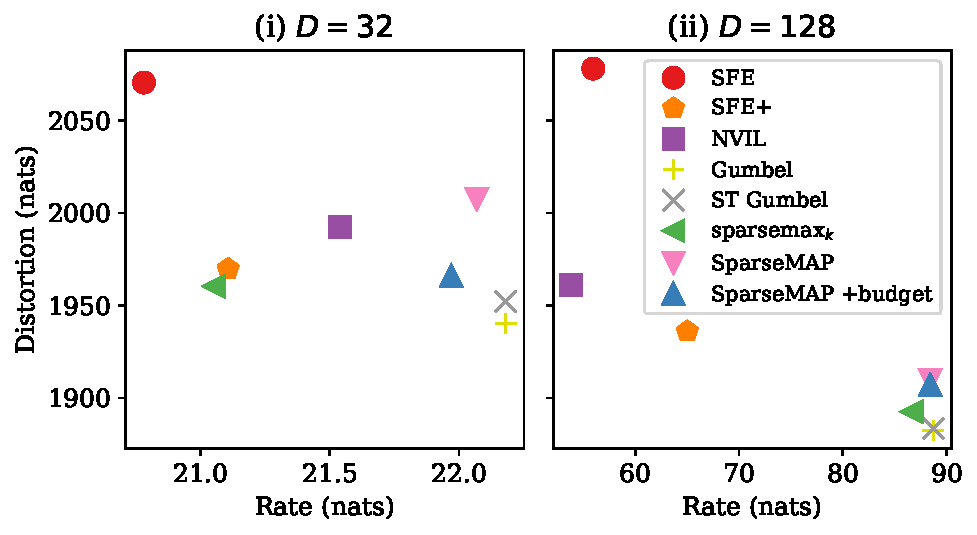
\includegraphics[width=0.95\textwidth]{Figures/distortion-rate.pdf}
    \caption[Test results for Fashion-MNIST.]{\label{fig:distortion_rd}Test results for Fashion-MNIST. RD plots
        (the closer to the lower right corner, the better).}
\end{figure}

\paragraph*{Results and discussion.} \tableref{tab:distortion_tab}
shows an importance sampling estimate ($1024$ samples per test
example were taken) of the negative log-likelihood for the several
methods, together with the converged values of each method in the RD
plane in \figref{fig:distortion_rd}. Both show results for which the
bit-vector has dimensionality $D=32$ and $D=128$. Regarding the
estimated negative log-likelihood, our methods exhibit increased
performance when compared to SFE, and top-$k$ sparsemax is
competitive with the remaining unbiased estimators. However, in the
RD plane, both our methods show comparable performance to SFE$+$ and
NVIL for $D=32$, but for $D=128$ all of our methods have a
significantly higher rate and lower distortion than any unbiased
estimator, suggesting a better fit of $p_X(x|\phi)$~\citep{Alemi2018}.
In \figref{fig:structcalls}, we can observe the training progress in
number of calls to $p_{X|Z}(x |z; \phi)$ for the models with 32 and 128
latent bits, respectively. While $\sparsemaxk$ introduces bias
towards the most probable assignments and may discard outcomes that
sparsemax would assign a non-zero probability to, as training
progresses distributions may (or tend to) be sufficiently sparse and
this mismatch disappears, making the gradient computation exact.

\begin{figure}[htbp]
    \centering
    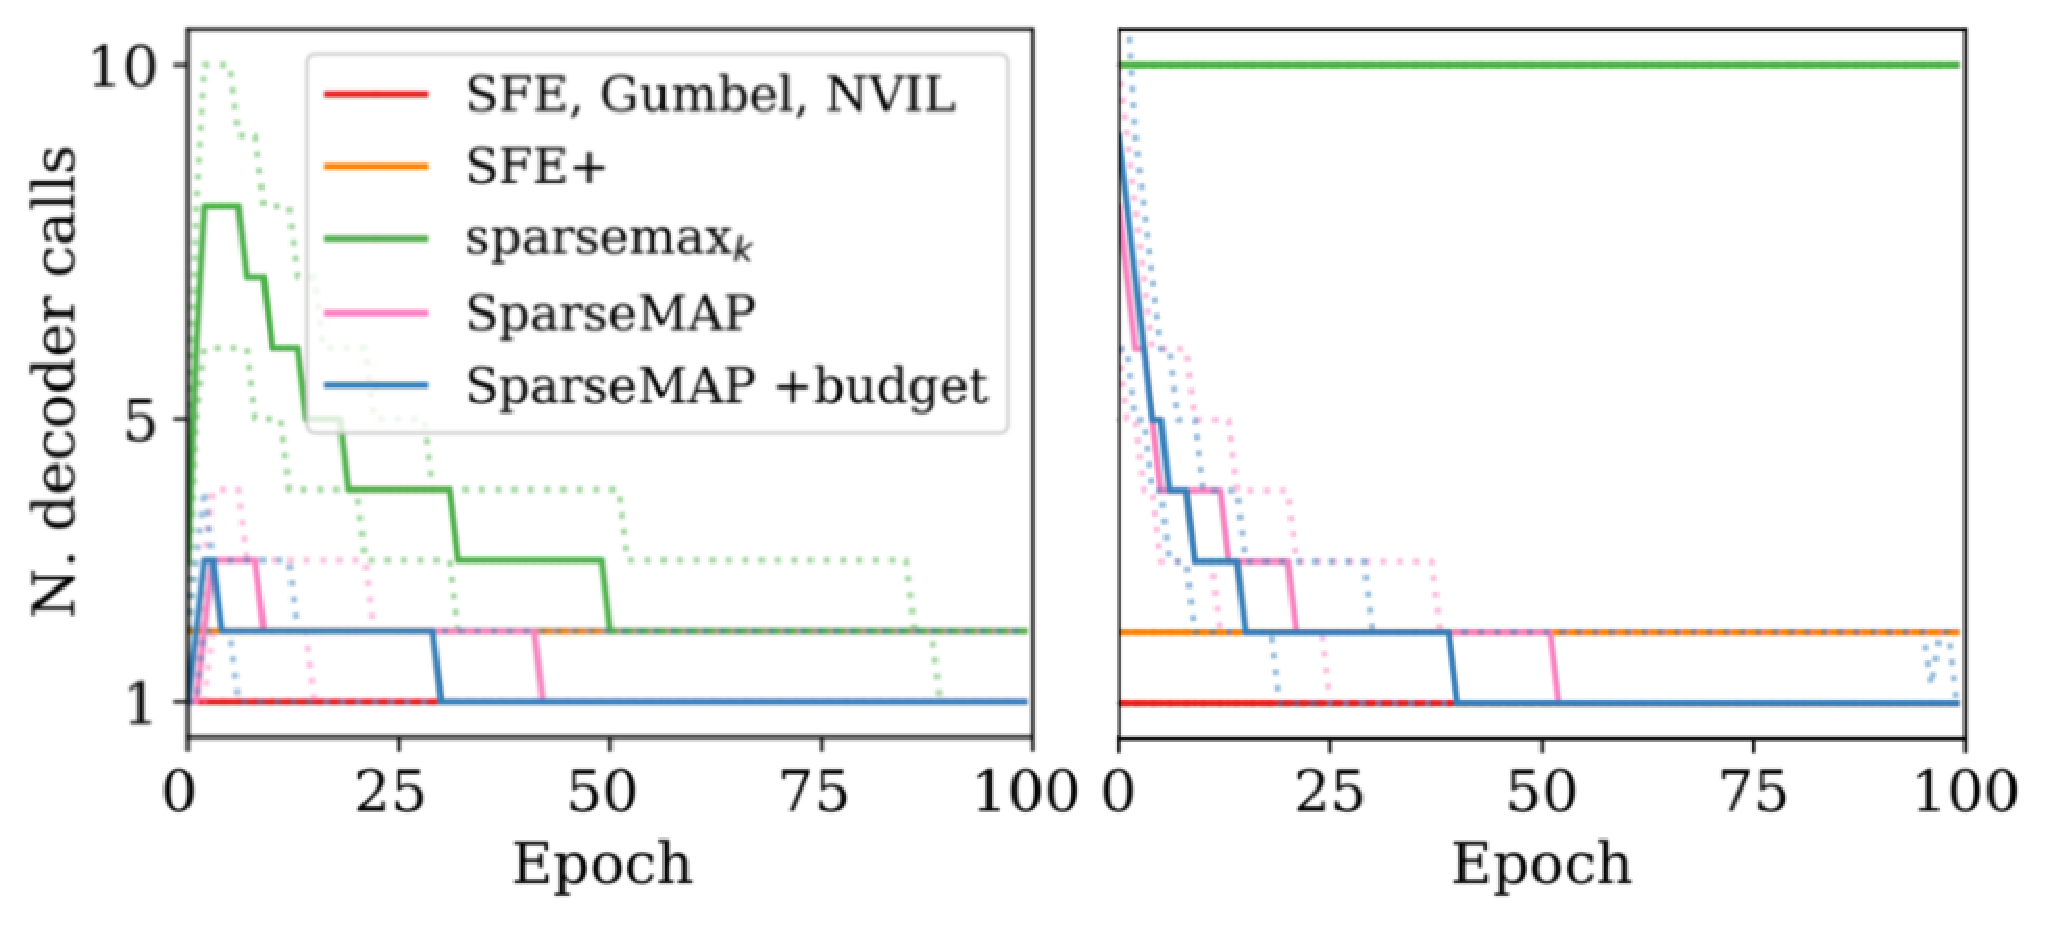
\includegraphics[width=0.95\textwidth]{Figures/spars.pdf}
    \caption[Bit vector VAE median and quartile decoder calls per
        epoch.]{Bit vector VAE median and quartile decoder calls per
        epoch,
        $D=32$ (left) / $D=128$ (right).\label{fig:structcalls}}
\end{figure}

Remarkably, this happens for $D\!=\!32$\,---\,the support of
$\sparsemaxk$ is smaller than $k$, giving the true gradient to
$q(z|x; \lambda)$ for most of the training. This no longer
happens for $D\!=\!128$, for which it remains with full support
throughout, due to the much larger search space. On the other hand,
\smap solutions become very sparse from the start in both cases,
while still obtaining good performance. There is, therefore, a
trade-off between the solutions we propose: on one hand,
$\sparsemaxk$ can become exact with respect to the expectation in
\eqnref{eq:fit}, but it only does so if the chosen $k$ is suitable to
the difficulty of the model; on the other hand, \smap may not offer
an exact gradient to $q(z|x; \lambda)$, but its performance is
very close to $\sparsemaxk$ and its higher propensity for sparsity
gifts it with less computation. \figref{fig:elbo_bit} shows the
downstream loss (ELBO) over epochs and over the median number of
decoder calls per epoch. The plots on \figref{fig:elbo_bit_calls}
show how our methods have comparable computational overhead to
sampling approaches. Oftentimes, our methods could have been trained
in fewer epochs to obtain the same performance as the sampling
estimators have for 100 epochs.

\begin{figure}[ht]
    \centering
    \begin{subfigure}[b]{0.49\textwidth}
        \centering
        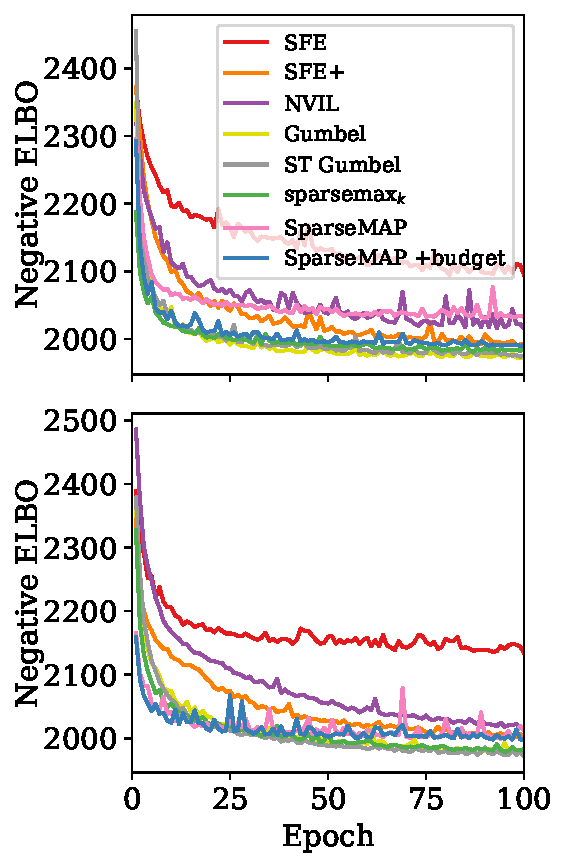
\includegraphics[width=\textwidth]{Figures/elbo-bit-vector.pdf}
        \caption{Neg. ELBO over training epochs.}
        \label{fig:elbo_bit_epochs}
    \end{subfigure}
    \begin{subfigure}[b]{0.49\textwidth}
        \centering
        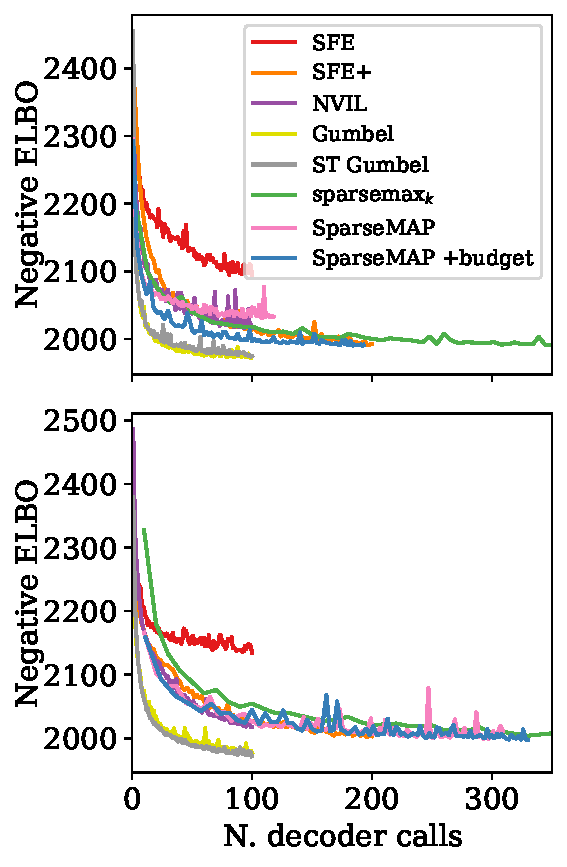
\includegraphics[width=\textwidth]{Figures/elbo-calls.pdf}
        \caption{Neg. ELBO over decoder calls.}
        \label{fig:elbo_bit_calls}
    \end{subfigure}
    \caption[Performance on the validation set
        for the experiment in \secref{sec:bernvae}.]{Performance on the validation set
        for the experiment in \secref{sec:bernvae},
        $D=32$ (top) / $D=128$ (bottom). For $D=32$, top-$k$ sparsemax continues
        until a total of 561 median decoder calls, and for $D=128$ it continues
        until a total of 998.}
    \label{fig:elbo_bit}
\end{figure}

Concerning relaxed estimators, note that the reconstruction loss is
computed given a continuous sample, rather than a discrete one,
allowing it more flexibility to directly reduce distortion and
potentially explaining why it does well in that regard. Moreover, the
rate of the relaxed model is unknown,\footnote{Estimating it would
    require a choice of Binary Concrete prior and an estimate of the KL
    divergence from that to the Binary Concrete approximate posterior
    \citep[Appendix C.3.2]{Concrete}.} and instead we plot the rate as if
$z$ was given discrete treatment, which, although common practice,
makes comparisons to other estimators inadequate. For ST
Gumbel-Softmax the situation is different since, after training, $z$
is given discrete treatment throughout. Its success shows that,
unlike in the other tasks considered, training on biased gradients is
not too problematic.

\section{Subsequent Work}
\label{sec:subsequent}

\noindent \citet{correia2020procneurips} proved to be a relevant
contribution to the field of discrete and structured latent variable
modeling. In particular, and most closely related to our work,
\citet{chen2021EvidentialSoftmaxSparse} added another method to the
family of efficient marginalization techniques that we started in
\citet{correia2020procneurips}. They introduce a new
function called \emph{ev-softmax} that has its origins in evidential
theory and evidential sparsification~\citep{itkina2020evidential}.
The properties of this function are more similar to \emph{softmax}
than \emph{sparsemax}, while still allowing for a sparse
distribution. They show that their method is less prone to
multimodality collapse~\citep{itkina2020evidential} and show improved
results in the experiment described in \secref{sec:gen}.

In another application of sparsity for discrete latent variable
models, \citet{farinhas2022SparseCommunicationMixed} introduced a new
family of mixed discrete-continuous random variables that can be used
to train these models. Their method has its origins in the recent
field of sparse and continuous
distributions~\citep{martins2020SparseContinuousAttention}. Their
method is applied to the experiments that we described in
\secref{sec:comm} and \secref{sec:bernvae} and show promising
results. As in our case, their method also bypasses the need for
methods with high variance, as in SFE, and relaxations of the
discrete space, as in Gumbel-Softmax; however, in their case, that's
not due to explicit marginalization but rather due to the nature of
the mixed random variables that they introduce.

As we will explore further in the next chapter, we believe that the
methods we have proposed here have potential for structured
applications. In particular, due to the structured nature of
language, the explicit marginalization of the structured space can
prove valuable to NLP. For example, our method has been applied
successfully for semantic
parsing~\citep{wang2021LearningExecutionsSemantic}. In this work, the
authors use our top-$k$ sparsemax method in the E-step of an EM
algorithm. Since they do not have access to a true top-$k$, they
approximate it using beam search. When compared to the other
baselines and other methods proposed, the approach that used top-$k$
sparsemax had the best performance.

\section{Final Remarks and Chapter Summary}

\noindent The solutions that were available to train discrete latent variable
models greatly relied on MC sampling, which can have high variance.
Methods that aim to decrease this variance are often not trivial to
train and implement and may disincentivize practitioners from
using this class of models. However, we believe that discrete latent variable models
have, in many cases, more interpretable, intuitive, and compact
latent representations.

We described a novel training strategy for discrete latent variable
models, eschewing the common approach based on MC gradient estimation
in favor of deterministic, exact marginalization under a sparse
distribution. Our training strategy offers: a simple approach in
implementation to training these models; no addition in the number of
parameters; low increase in computational overhead (especially when
compared to more sophisticated methods of variance
reduction~\citep{RB19}); and improved performance.
Sparsity leads to a powerful \textbf{adaptive} method,
which can investigate fewer or more latent assignments $z$ depending
on the ambiguity of a training instance $x$, as well as on the stage
in training.

We showcase the performance and flexibility of our
methods by investigating a variety of applications, with both discrete
and structured latent variables, with positive results. Our models
very quickly approach a small number of latent assignment evaluations
per sample, but make progress much faster and overall lead to
superior results.

Our proposed method thus offers the accuracy and robustness of exact
marginalization while meeting the efficiency and flexibility of sampling
methods, providing a promising alternative to
successfully train more \textbf{compact} neural models. As we are
learning from subsequent works (\secref{sec:subsequent}), we believe
that our method can be used to address the challenges of training
these sorts of models in a variety of applications, particularly NLP.

\cleardoublepage

\singlespacing